\section{Importing textual use-case specifications into the \emph{Reprotool} project}

In this section we are going to explore the feature of the \emph{Reprotool IDE} that enables you to type the use-cases in a text
editor and later import them into a \emph{Reprotool} project. Firstly, we will show you an example of a textual specification
of use-cases in \emph{Reprotool}. After you look at it and get the general idea of how it works, we will explain in detail how you can
create your own textual use-case specifications.

\subsection{The Admission system example project}

The \emph{Adminnsion system} example project is part of the \emph{Reprotool exmaple projects}. If you have not installed them
already into your workspace, please do it now using the following instructions. Use this command:
\begin{verbatim}
File / New / Example... /
\end{verbatim}

Now select the \emph{Reprotool exmples} in the \emph{Reprotool} category. Now click Finish. All of the \emph{Reprotool} example projects
should be installed in your workspace now. Look for the \emph{Admission system} project.
It contains an empty project and the \emph{data} directory where the textual use-case specifications are stored. If you double-click one
of these files, you will be asked if you want to add the \emph{Xtext} nature into your project. Please, choose yes. Now please take a
while and browse these files until you get a general idea about the format of these use-case specifications.

\subsection{Importing the use-cases into a reprotool project}

Now we are going to import these textual specifications into the empty \emph{Admission system} project. Firstly open the
\emph{admission.swproj} file in the \emph{Admission system} exmaple project. You should see that this project does not contain any
use-cases yet. Luckily, we are going to change it. Choose the following command:
\begin{verbatim}
File / Import
\end{verbatim}

Now select the \emph{Reprotool} category and the \emph{Import use-cases} wizard. Now you should see a window similar to this:

\newpage

\begin{figure}[ht]
  \centering
  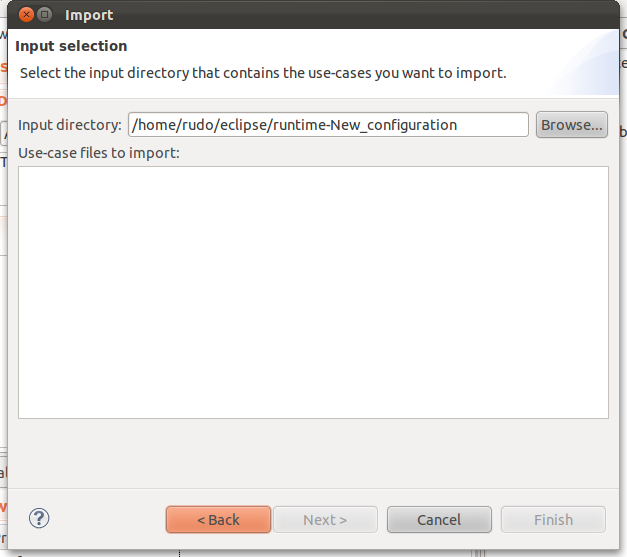
\includegraphics[height=280pt]{images/reprotoolImportWizard}
  \caption{Reprotool import wizard}
  \label{fig:reprotoolImportWizard}
\end{figure}

Here you are asked to provide the input data for your import. Click the \emph{Browse} button and select the \emph{data} directory
in the \emph{Admission system} project.

Click \emph{Next}. In the next window, you are asked to specify the output of the import process. Make sure that the radio box
\emph{Import use-cases into an existing project} is checked and click the \emph{Browse} button. Now browse for the
\emph{admission.swproj} file in the \emph{Admission system} project directory. And click the \emph{Finish} button. The project
editor window automatically reloads its contents and now you can see the imported use-cases.
